SVR PF
Lo mas simple es promediar ambas predicciones y ver los resultados.

Usar SVR para predecir el valor y hacer correcciones con PF. Mover las particulas dependiendo de las predicciones de SVR

Usar SVR dentro de la funcion de movimiento de las particulas. Puede ser predecir la tasa de cambio del siguiente paso y que las particulas se muevan segun ese valor.




\begin{table}
\caption{Table captions should be placed above the
tables.}\label{tab1}
\begin{tabular}{|l|l|l|}
\hline
Heading level &  Example & Font size and style\\
\hline
Title (centered) &  {\Large\bfseries Lecture Notes} & 14 point, bold\\
1st-level heading &  {\large\bfseries 1 Introduction} & 12 point, bold\\
2nd-level heading & {\bfseries 2.1 Printing Area} & 10 point, bold\\
3rd-level heading & {\bfseries Run-in Heading in Bold.} Text follows & 10 point, bold\\
4th-level heading & {\itshape Lowest Level Heading.} Text follows & 10 point, italic\\
\hline
\end{tabular}
\end{table}


\begin{figure}
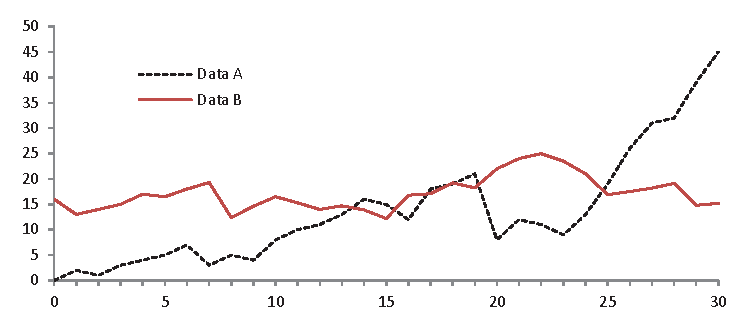
\includegraphics[width=\textwidth]{fig1.eps}
\caption{A figure caption is always placed below the illustration.
Please note that short captions are centered, while long ones are
justified by the macro package automatically.} \label{fig1}
\end{figure}

The remaining of this paper is structured as follows: Section \ref{sec:related_work} extend the background of this work and explains similar works to the one proposed in this study. Section \ref{sec:material_method} describes the metrics, data sets and overviews the proposed approach used in this study. Section \ref{sec:results} gathers the main results obtained from the experiments. Section \ref{sec:disscussion} explores the significance of the work's results. Finally, the concluding remarks are drawn in Section \ref{sec:conclusions}. 